%%%%
% -- Instrument Description
% --     FOBOS Keck White Paper 2019
%%%%


\section{Instrument Overview}
\label{sec:concept}
% \noindent \comment{1 page}

% Here's an alternative way to put in figures if we want captions on the side (to save space)
% Could introduce a new ``counter'' to count and label figures appropriately
%\centerline{\hbox{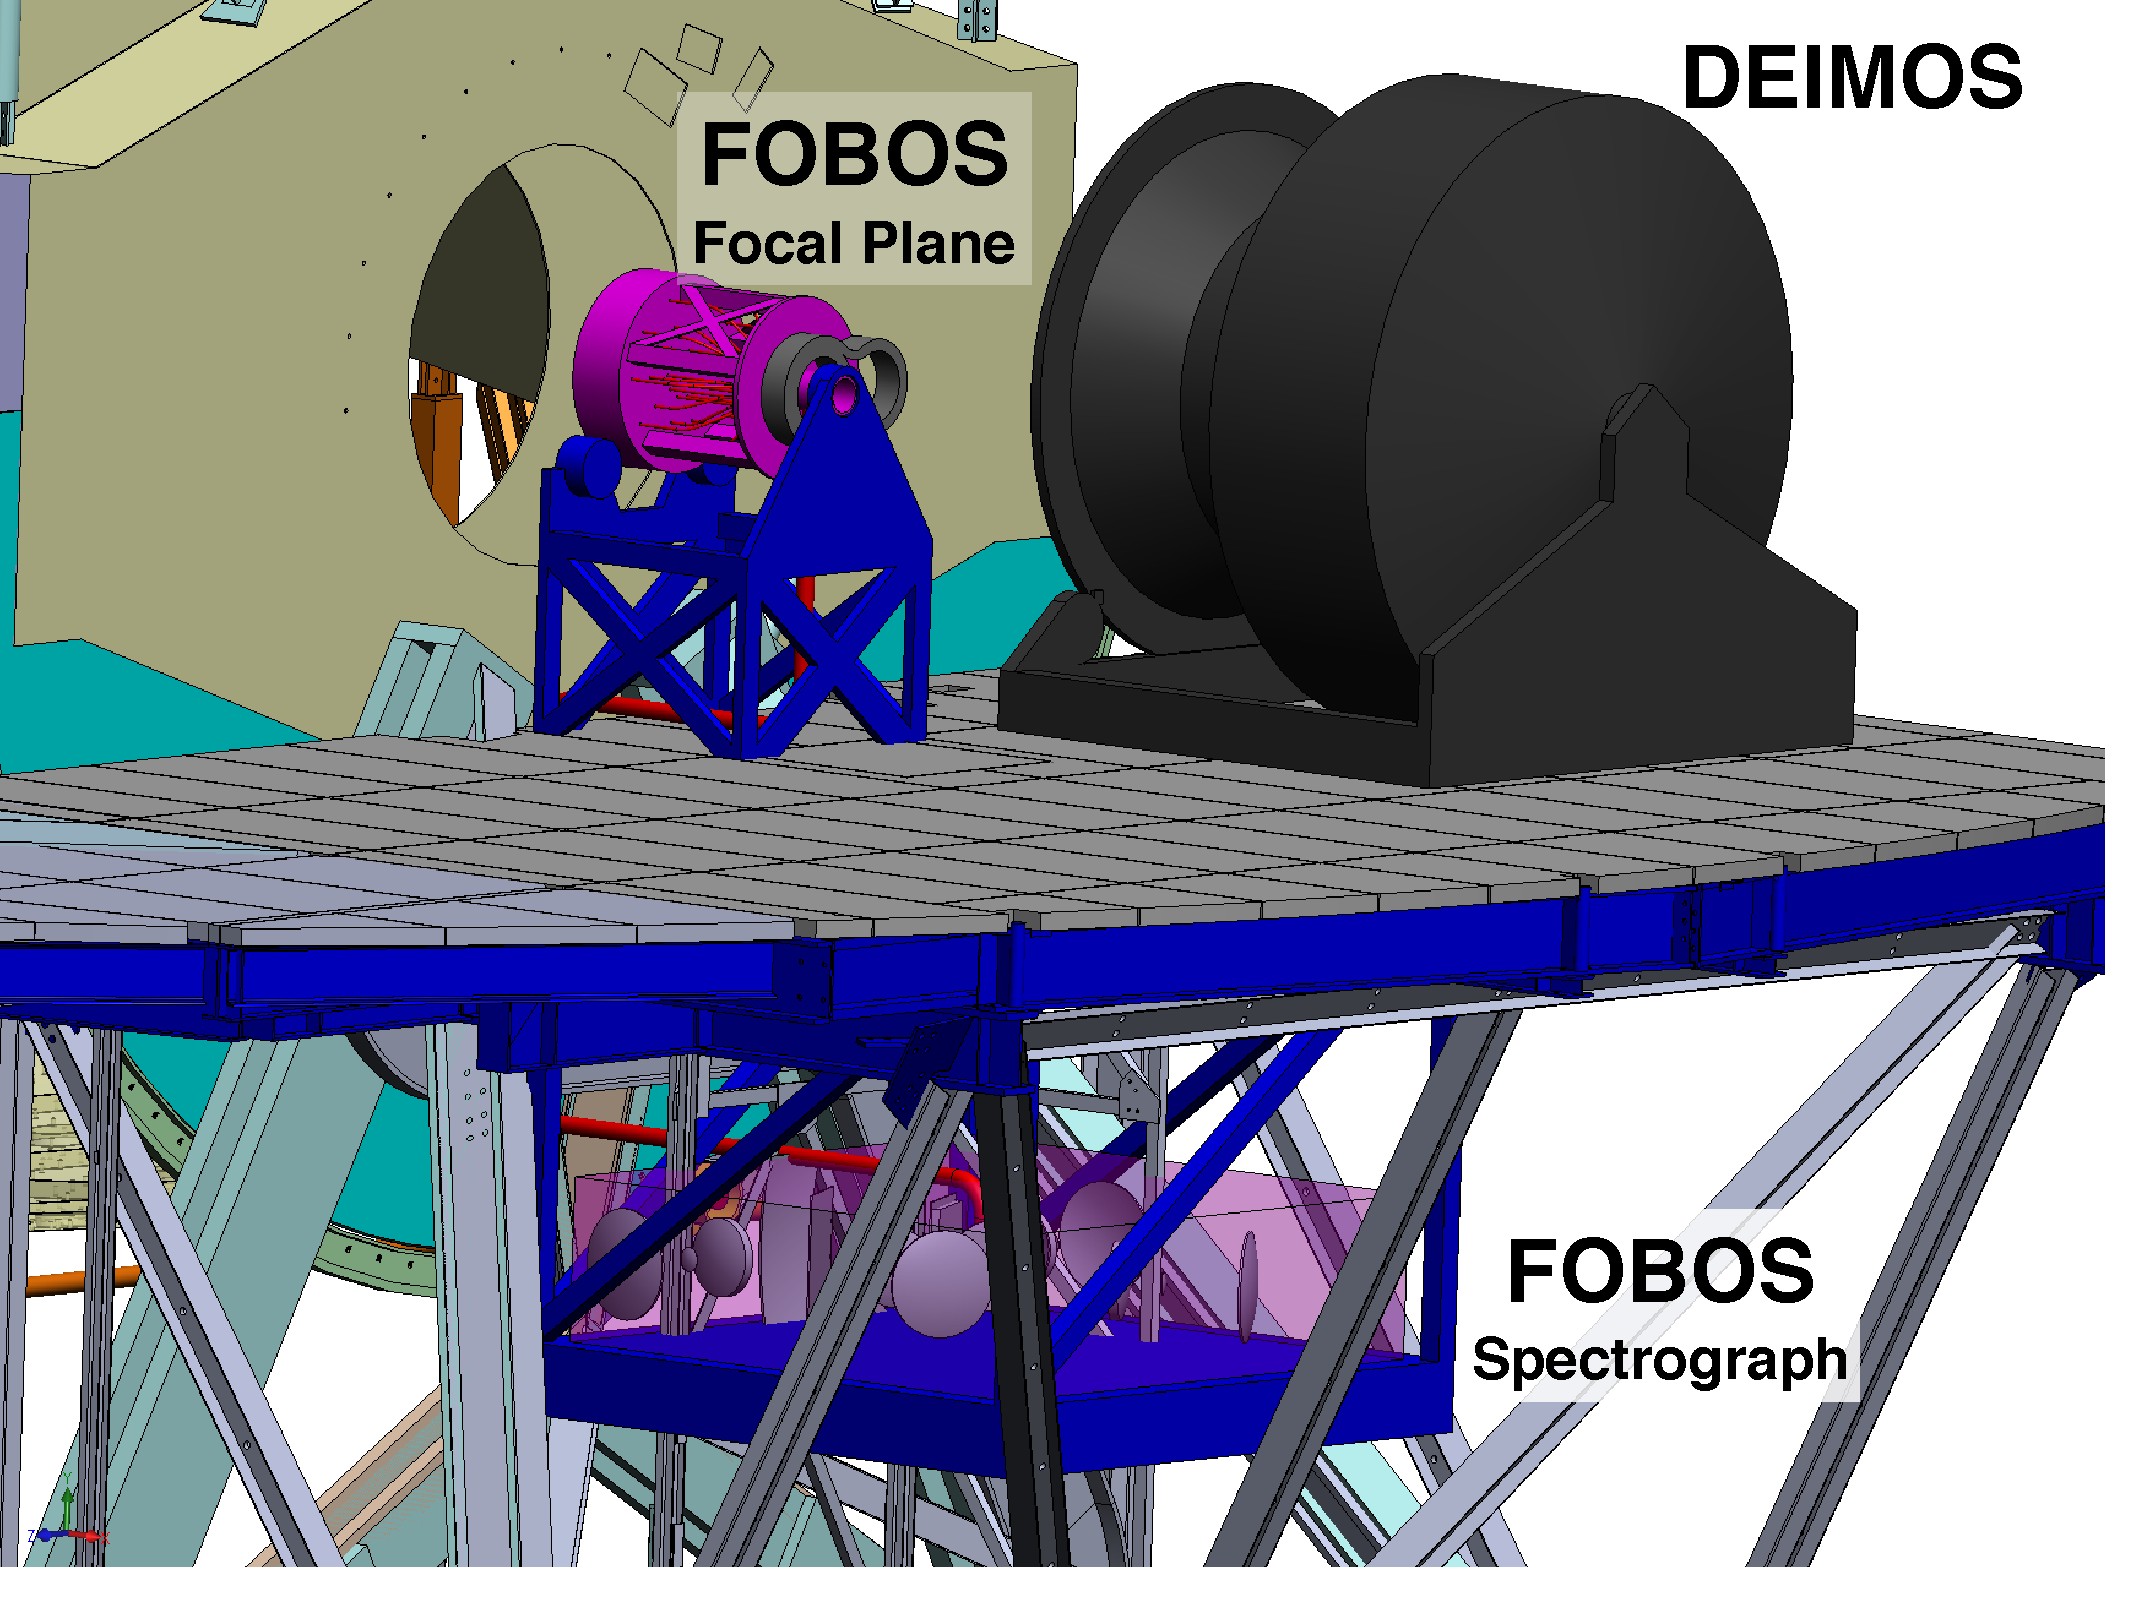
\includegraphics[width=0.6\textwidth, angle=0]{figs/FOBOSatKeck_v1.pdf}
%    \hspace{0.1cm} \vspace{2in}
%    \parbox[b]{0.3\textwidth}{\small {\bf Figure ??:} Rendering of FOBOS instrument systems deployed at the Keck II Nasmyth port.  By mounting the FOBOS spectrographs under the Nasmyth platform, other instruments like DEIMOS can maintain access to the telescope. \vspace{2cm}}}}

%%%%%%%%%%%%%%%%%%%%%%%%%%%%%%%%%%%%%%%%%%%%%%%%%%%%%%%%%%%%%%%%%%%%%%%%
\begin{figure}[h!]
\vskip -0.1in
%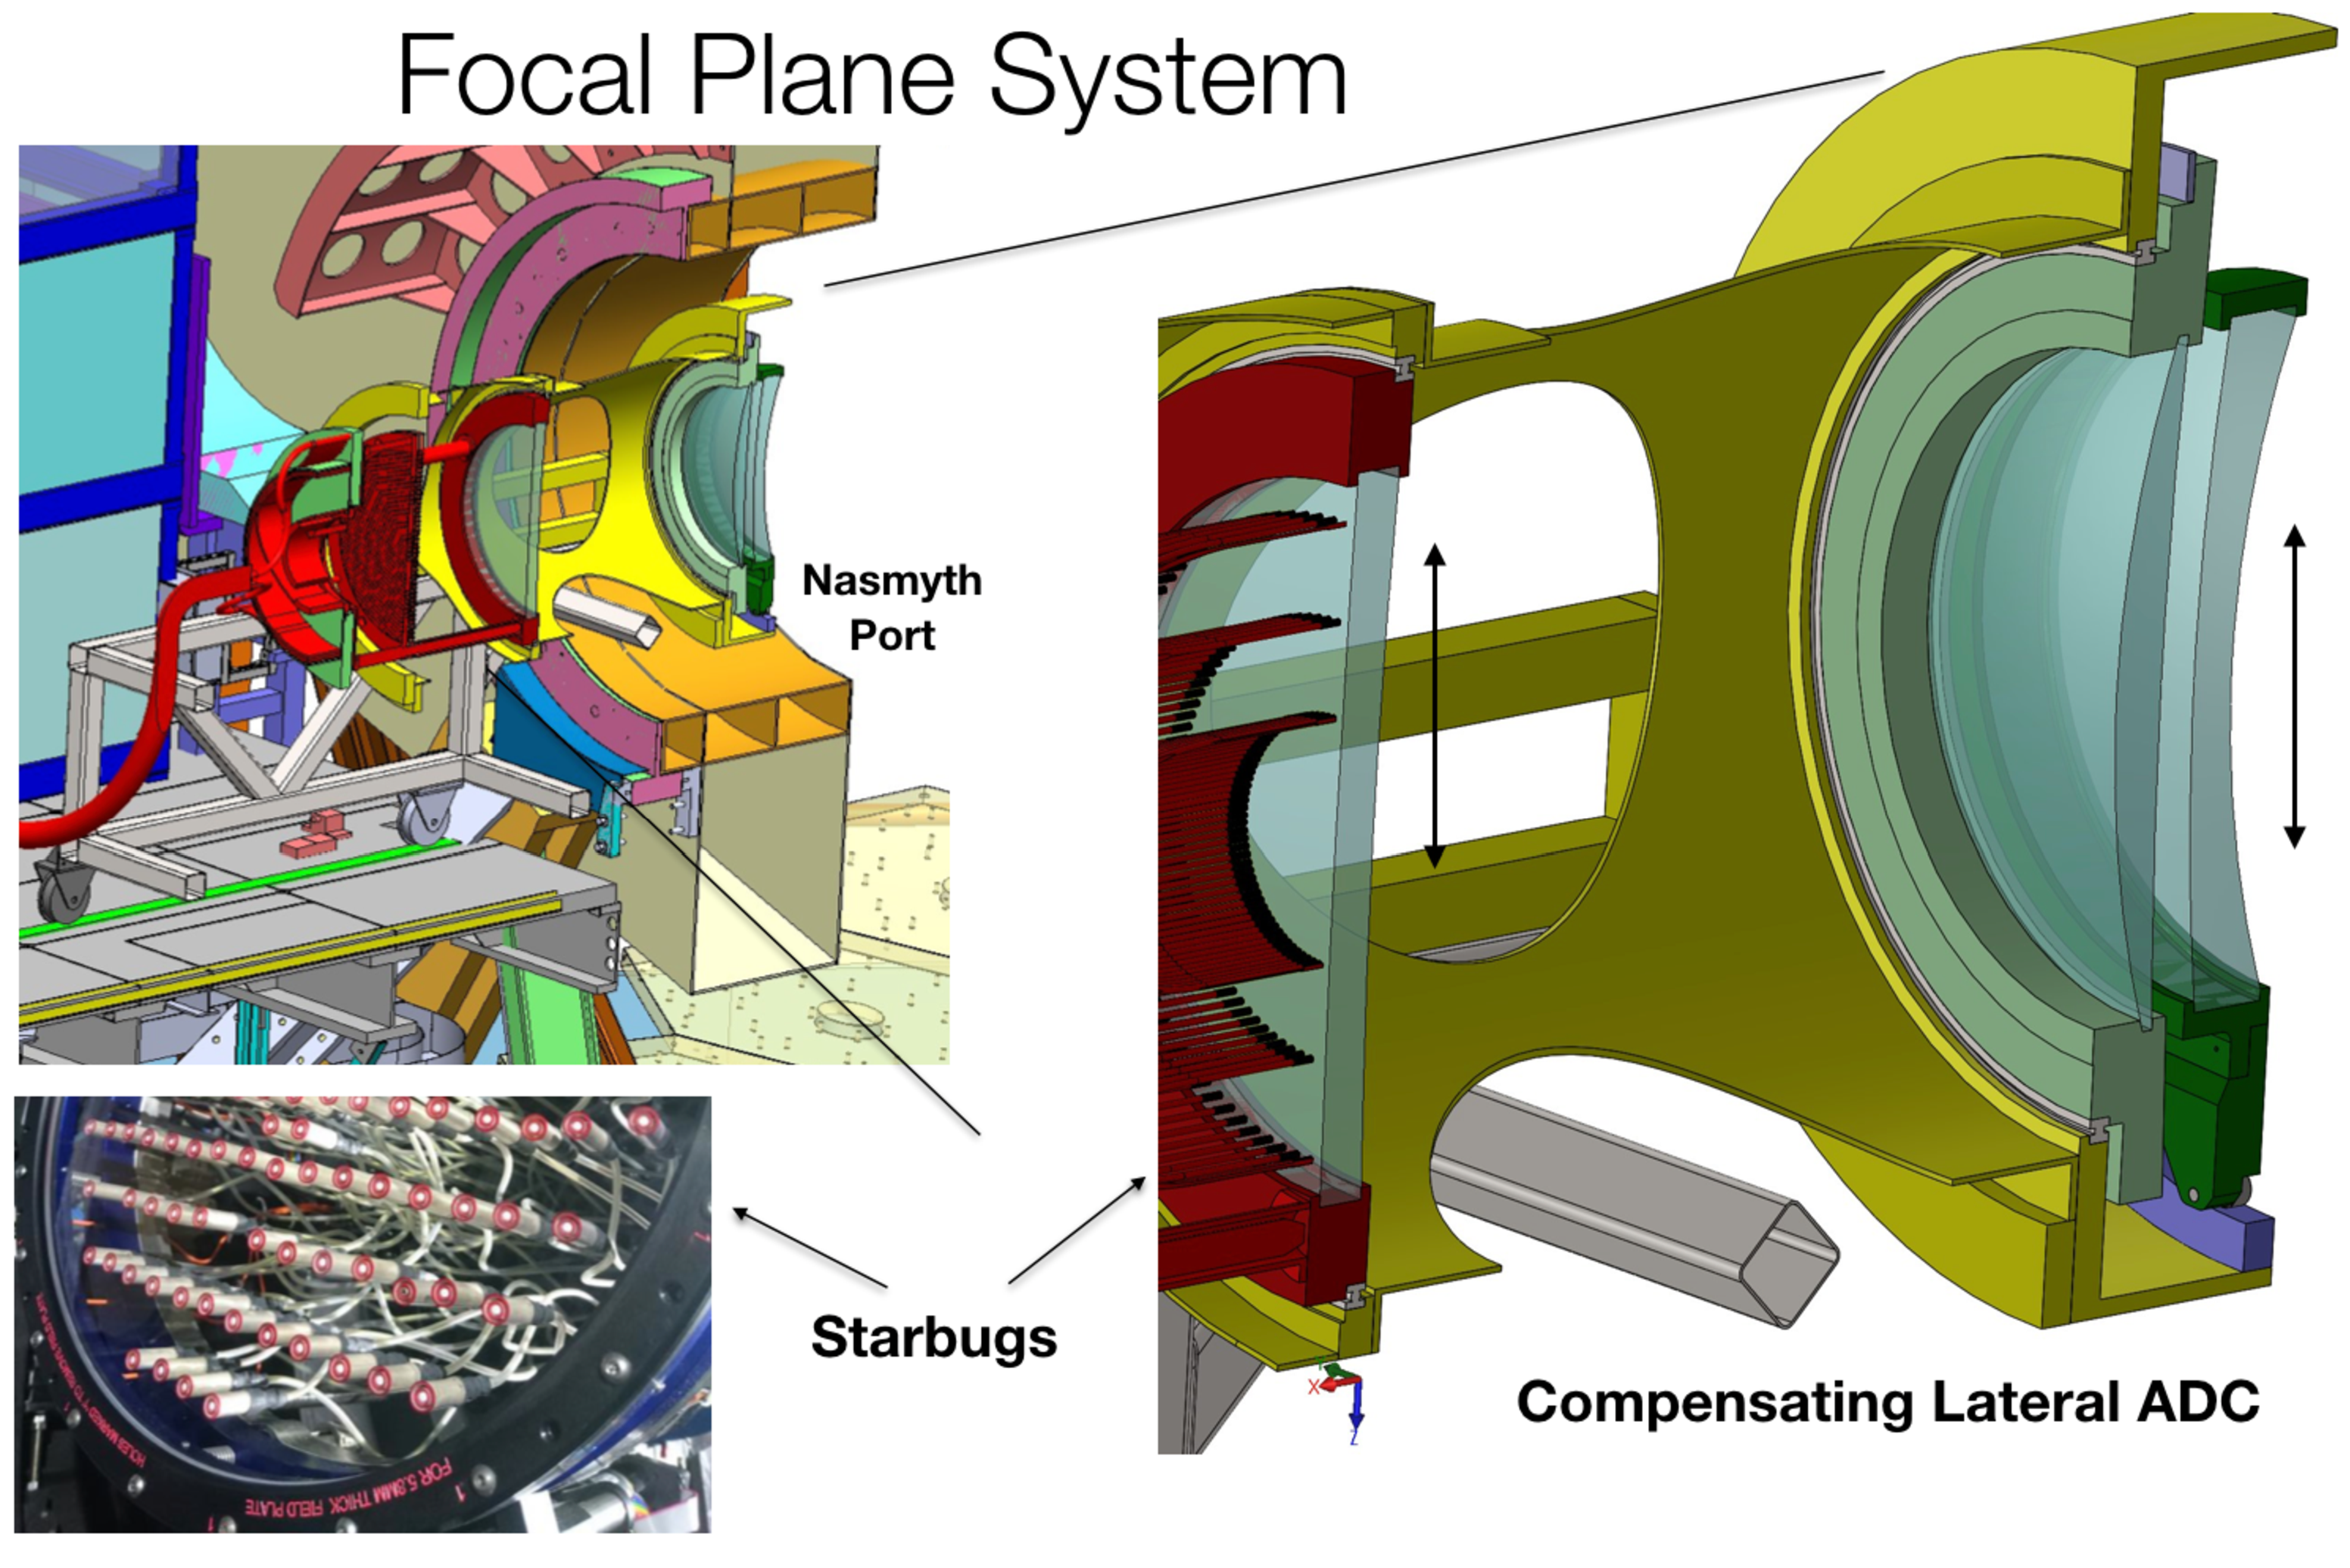
\includegraphics[width=\textwidth]{figs/FOBOS_FocalPlane.pdf}
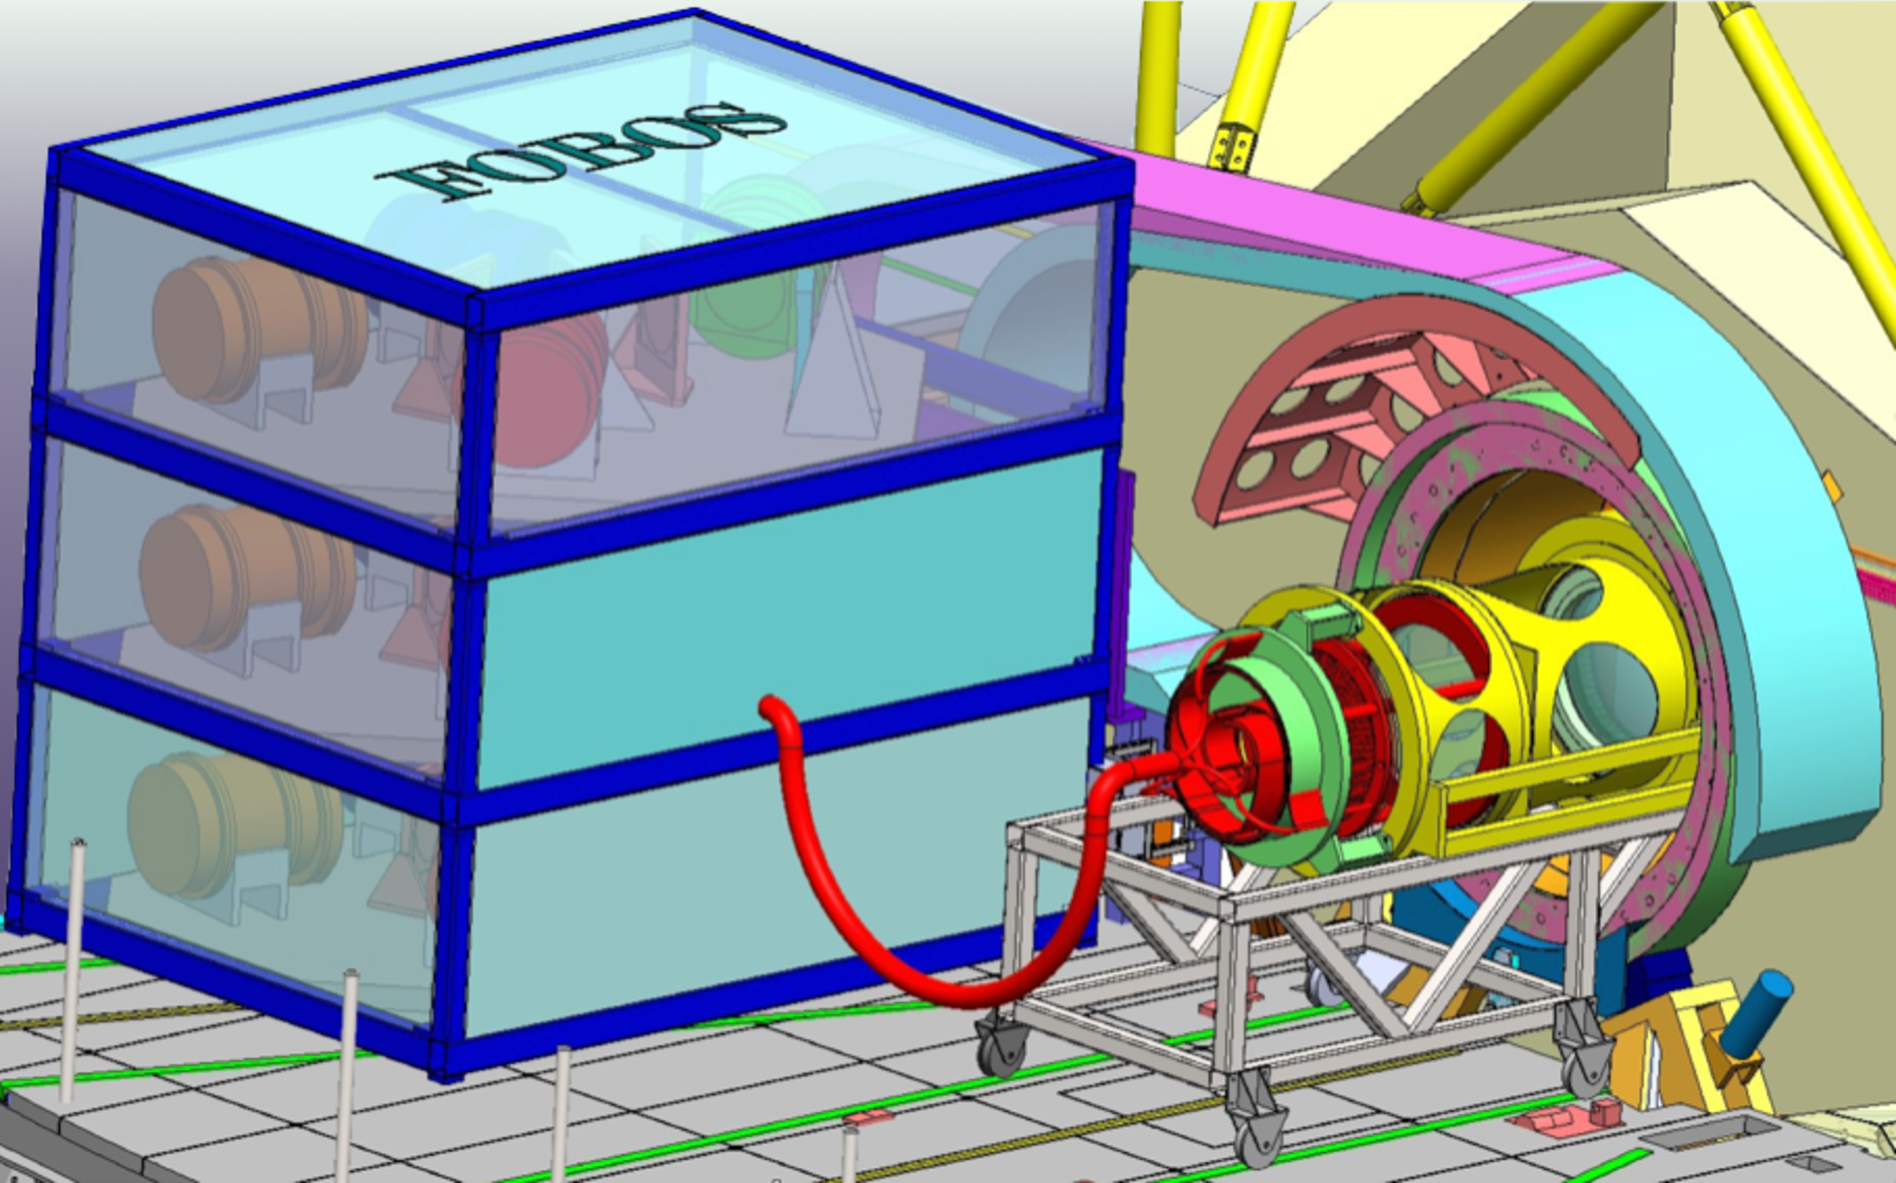
\includegraphics[width=\textwidth]{figs/FOBOS_inst_v2.pdf}
\caption{\small \comment{Changed figure to get it to compile.} {\it
Left}: Rendering of FOBOS focal plane system deployed at the Keck II
Nasmyth port. By mounting the FOBOS spectrographs under the Nasmyth
platform, other instruments like DEIMOS can maintain access to the
telescope. {\it Right}: Rendering of the ADC and focal surface with
Starbugs mounted (red cylinders). {\it Bottom-left}: Starbugs
deployed on the TAIPAN instrument.}
\label{fig:focalplane}
\end{figure}
%%%%%%%%%%%%%%%%%%%%%%%%%%%%%%%%%%%%%%%%%%%%%%%%%%%%%%%%%%%%%%%%%%%%%%%%

Mounted at the Nasmyth focus of Keck II Telescope at WMKO, FOBOS
(Figure \ref{fig:layout}) will be one of the most powerful
spectroscopic facilities deployed in the next decade. FOBOS includes
a compensating lateral atmospheric dispersion corrector (CLADC, not
pictured) to ensure that target light from all wavelengths falls on
allocated fibers while also correcting image aberrations at the edges
of the 20-arcmin diameter Keck field. Each of the CLADC lenses is 946
mm in diameter, the first two are closely spaced with lateral
relative motions enabled by three barrel-mounted actuators. The final
CLADC lens surface translates to track focal plane tilt, and it
serves as the vertical mounting plate for roaming Starbugs fiber
positioners \comment{ref}. Starbugs patrol a large on-sky area
($\sim$1 arcmin), enabling flexible and dynamic targeting
configurations with adjacent fibers as close as 10 arcsec.

% How much do we go into risks?

A total of 1800 fibers with 150-$\mu$m core diameter are deployed at
the curved focal plane. Microlens fore-optics convert the f/15 Keck
input beam to a faster f/3 focal ratio, which both demagnifies the
entrance aperture and allows for better coupling to the fiber
numerical aperture by minimizing losses from focal ratio degradation.
The focal-plane plate rotates and translates to follow image
positions as the telescope tracks across the sky. The fiber run is
kept at less than 10m to maintain high throughput at UV wavelengths
(a 10m Polymicro Silica fiber transmits $\sim$70\% and $\sim$85\% of
light at 310nm and 350nm, respectively). Special care is given to
stress-relief cabling to minimize instabilities (e.g., variable focal
ratio degradation) over the fiber run.

Sets of 600 fibers feed each of three identical spectrographs (Fig
\ref{fig:layout}). Each spectrograph uses a series of dichroics to
divide the 259mm-diameter collimated beam into four wavelength
channels, providing an instantaneous broad-band coverage from 0.31--1
$\mu$m. Fused-silica etched (FSE) gratings provide mid-channel
spectral resolutions of $R \sim 3500$ at high diffraction efficiency
in each channel. The dispersed light is focused by an f/1.1
catadioptric camera\footnote{Based on the camera design for the
Multi-Object Optical and Near-infrared Spectrograph (MOONS) on the
Very Large Telescope (VLT).} and recorded by an on-axis 4k$\times$4k
CCD mounted at the center of the first camera lens element.
Spectrographs are mounted in a permanent temperature-controlled
housing on the Nasmyth deck, whereas the focal-plane system can be
unmounted and stowed alongside existing Keck instruments. The
end-to-end instrument throughput peaks at 60\% and is greater than
30\% at {\it all} wavelengths.

FOBOS includes observatory level systems for precise instrument
calibration using dome-interior screen illumination, a metrology
system for accurate fiber positioning, and guide cameras for field
acquisition and guiding. \comment{make the following consistent with
what we say in the summary}. Initial deployment of the focal-plane
will focus on a single-fiber format, with a secondary deployment of
multi-format fiber bundles to follow. Additional instrument upgrades
include integration of fibers that feed additional spectographs ---
these spectrographs could provide increased multiplex capacity,
higher spectral resolution, and/or observe different spectral regions
--- and additional front-end sensing equipment that fully support and
benefit from image corrections with Ground-Layer Adaptive Optics.
